\chapter{Design of Cloud-SAP}

\chapterintro{ This chapter introduces the high-level design of Cloud-SAP.
  Further elaboration on the layers of the proposed platform is presented
  and detailed discussion about the each layer is held.
}

\section{Requirements}
One can notice that elements that yields a solution for a problem stated in the first chapter, which is ensuring that users' application provide appropriate Quality-of-Service for its customers in a most-cost effective manner, were gradually introduced in previous chapters:

\begin{itemize}
	\item \emph{scalability} - ability to improve application performance by enriching resources
	\item \emph{adaptivity} - ability to adapt (i.e. scale) appropriately to a current usage pattern
	\item \emph{inter-cloud awareness} - ability to compose an application deployment using different cloud providers; cooperation with different cloud provider to supply application with extra resources while performing application scaling
\end{itemize}

Next section states the general overview of the proposed solution, while the consecutive sections presents more detailed discussion of its elements and finally the last section summarises the design choices in a context of system requirements.
	
\section{High-level design}
\subsection{Overview}

\begin{figure}[!ht]
  \begin{center}
    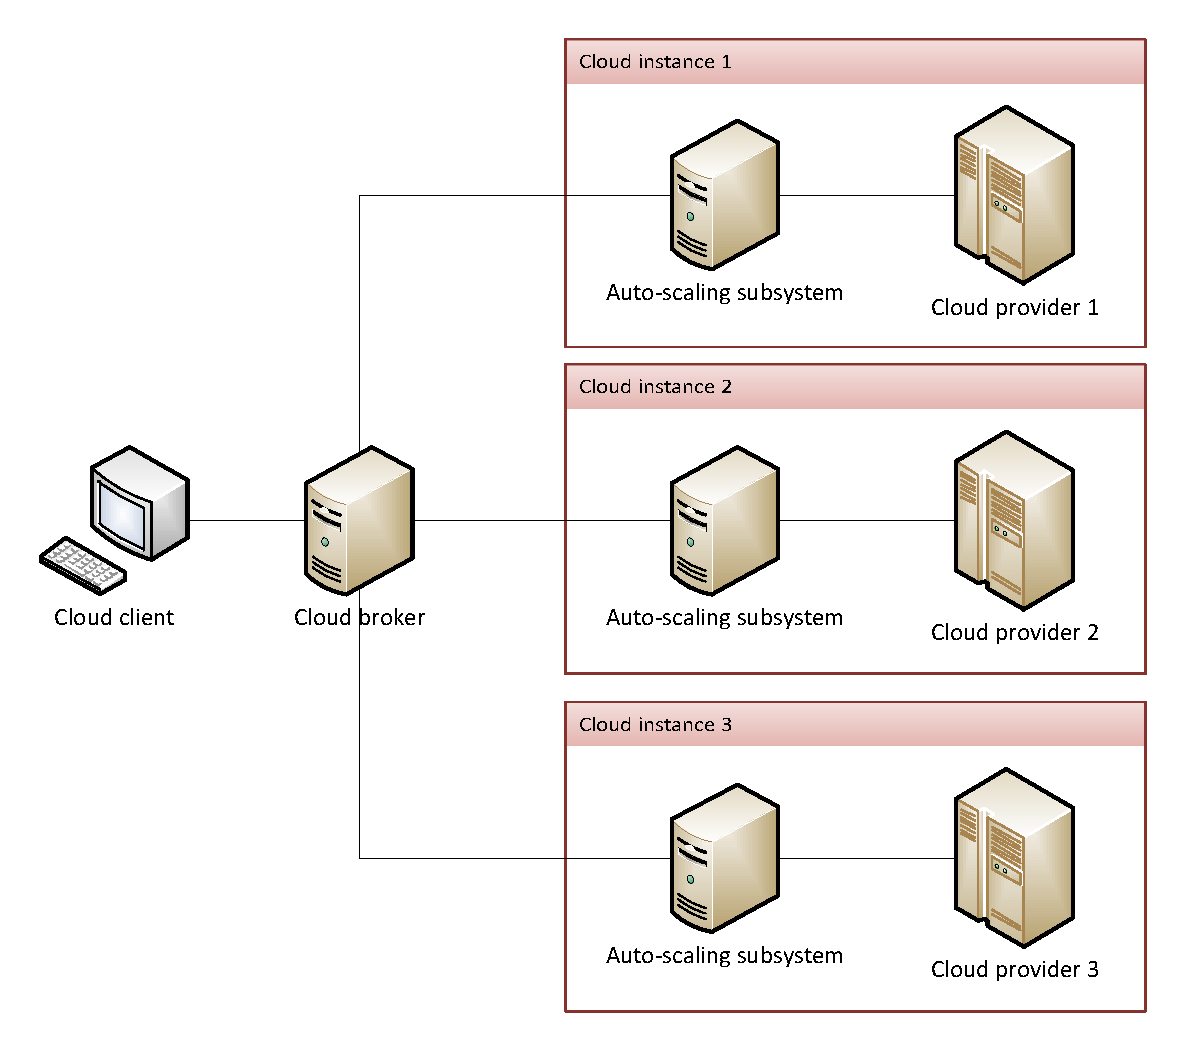
\includegraphics[width=0.8\textwidth]{chapter-5/hld-overview}
  \end{center}
  \caption{Cloud-SAP high level overview}
  \label{design:hld-overview}
\end{figure}

As diagram \ref{design:hld-overview} illustrates, we can distinguish two main components of proposed solution: auto-scaling module and inter-cloud broker. Together, they can be seen as an hierarchical autonomic system, where each layer corresponds to a different scalability perspective:
\begin{itemize}
	\item application platform layer: application platform tuning
	\item container layer: vertical scaling
	\item stack layer: horizontal scaling
	\item inter-cloud layer: scaling out across different cloud providers
\end{itemize}

Diagram \ref{design:csap-layers} depicts that multi-layered structure.

\begin{figure}[!ht]
  \begin{center}
    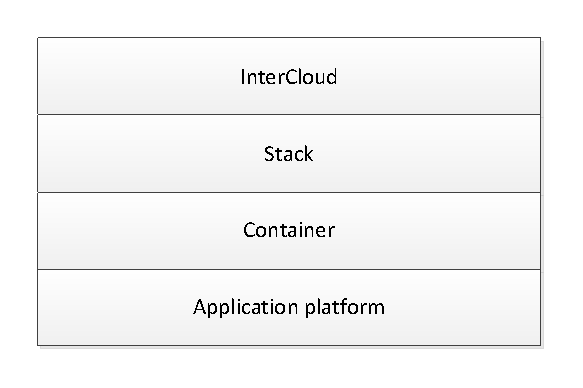
\includegraphics[width=0.5\textwidth]{chapter-5/sap-layers}
  \end{center}
  \caption{Layered structure of Cloud-SAP}
  \label{design:csap-layers}
\end{figure}

\subsection{Auto-scaling module}

\subsubsection{Autonomic components}
Each layer of the Cloud-SAP (shown in figure \ref{design:csap-layers}) must be characterised by an ability to adapt to a given application usage. As the previous chapter stated, this can be achieved by adding an elasticity controller to each layer. This observation is a foundation of proposed architecture.

One of the first models that ensured system adaptivity is an autonomic component, concept based on a feed-back loop, initially proposed by IBM \cite{IBM06}. Figure \ref{design:autonomic-component} depicts that architecture. 

\begin{figure}[!ht]
  \begin{center}
    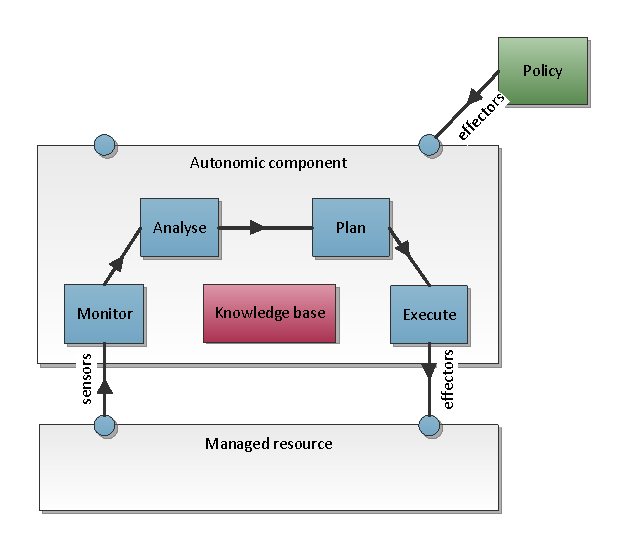
\includegraphics{chapter-5/autonomic-component}
  \end{center}
  \caption{autonomic component}
  \label{design:autonomic-component}
\end{figure}

Since designed platform operates on multiple layers, we can extend that model by using concept of a multi-hierarchical autonomic system \cite{LiWoZh05}. Figure \ref{design:hierarchical-autonomic-system} illustrates that hierarchy, were each level represents a different perspective on an application scaling. Using terminology characteristic to a autonomic system, first three hierarchy levels (application tuning, container, stack) are centralised and controlled by a single elasticity controller at each level, while the last inter-cloud level is a decentralized one - each cloud instance is fully independent.

\begin{figure}[!ht]
  \begin{center}
    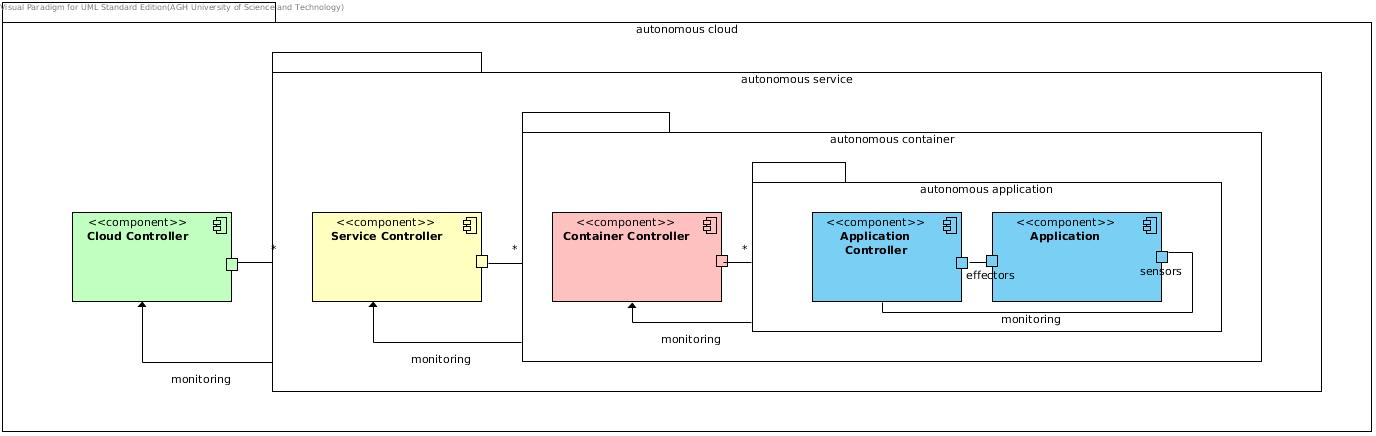
\includegraphics[width=0.8\textwidth]{chapter-5/hierarchical-autonomic-system}
  \end{center}
  \caption{Cloud-SAP as an hierarchical autonomic system}
  \label{design:hierarchical-autonomic-system}
\end{figure}

As \cite{IBM06} states, each autonomic component has modules that are responsible for:
\begin{itemize}
	\item monitoring
	\item analysis
	\item planning
	\item action execution
\end{itemize}

While the managed component has:
\begin{itemize}
	\item sensors
	\item effectors
\end{itemize}

Due to the hierarchy of our architecture, each level manages an underlying autonomic component, while being managed by an upper layer at the very same time.

\subsubsection{Monitoring}

\subsubsection{Analysis}

\subsubsection{Planning}

\subsubsection{Execution}


\subsection{Cloud federation}
Opis najwyzej warstwy, ze ma brokery, wykorzystuje kilka chmur.


\section{Auto-scaling module}

\section{Cloud federation}

\section{Solution discussion}
